\documentclass[10pt,a4paper]{article}

%%%%%%%%%%%%%%%%%%%%%%%%%%%
% MODIFY:

\newcommand{\authorA}{Jia Long Ji Qiu}
\newcommand{\authorB}{Jiabo Wang}
\newcommand{\authorC}{Yilun Liu}
\newcommand{\groupNumber}{J} % - YOUR GROUP NUMBER
\newcommand{\exerciseNumber}{5} % - THE NUMBER OF THE EXERCISE
\newcommand{\sourceCodeLink}{https://github.com/jialongjq/mlcms}

\newcommand{\workPerAuthor}{
\authorA&Task 1&1/3\\
      &Task 2&1/3\\
      &Task 3&1/3\\
      &Task 4&1/3\\
      &Task 5&1/3\\
      \hline
\authorB&Task 1&1/3\\
      &Task 2&1/3\\
      &Task 3&1/3\\
      &Task 4&1/3\\
      &Task 5&1/3\\
      \hline
\authorC&Task 1&1/3\\
      &Task 2&1/3\\
      &Task 3&1/3\\
      &Task 4&1/3\\
      &Task 5&1/3\\
}

%%%%%%%%%%%%%%%%%%%%%%%%%%%

%%
% imports for the exercise sheets
%

\usepackage[utf8]{inputenc}
\usepackage{amsmath}
\usepackage{amsfonts}
\usepackage{amssymb}

\usepackage[yyyymmdd]{datetime}
\renewcommand{\dateseparator}{--}

\usepackage[left=2cm,right=2cm,top=3cm,bottom=3cm]{geometry}
\usepackage{listings, xcolor}

\definecolor{codegreen}{rgb}{0,0.6,0}
\definecolor{codegray}{rgb}{0.5,0.5,0.5}
\definecolor{codepurple}{rgb}{0.58,0,0.82}
\definecolor{backcolour}{rgb}{0.95,0.95,0.92}

\lstdefinestyle{mystyle}{
    backgroundcolor=\color{backcolour},   
    commentstyle=\color{codegreen},
    keywordstyle=\color{magenta},
    numberstyle=\tiny\color{codegray},
    stringstyle=\color{codepurple},
    basicstyle=\ttfamily\footnotesize,
    breakatwhitespace=false,         
    breaklines=true,                 
    captionpos=b,                    
    keepspaces=true,               
    showspaces=false,                
    showstringspaces=false,
    showtabs=false,                  
    tabsize=2
}

\lstset{style=mystyle}

\usepackage{hyperref}

\usepackage{amsthm}
\newtheorem{lem}{Lemma}
\newtheorem{thm}{Theorem}
\newtheorem{cor}{Corollary}
\newtheorem{rem}{Remark}
\newtheorem{definition}{Definition}
\newtheorem{ter}{Terminology}

\usepackage{graphicx}

\newcommand{\M}{\mathcal{M}}
\newcommand{\N}{\mathcal{N}}
\newcommand{\K}{\mathcal{K}}
\newcommand{\SPDk}{\mathbb{P}^k}
\newcommand{\vol}{\text{vol}}

\newcommand{\Figref}[1]{Figure~\ref{#1}}
\newcommand{\figref}[1]{figure~\ref{#1}}
\newcommand{\Eqnref}[1]{Equation~(\eqref{#1})}
\newcommand{\eqnref}[1]{equation~(\eqref{#1})}

\usepackage{float}
\usepackage{tabularx}

\usepackage{fancyhdr}
\pagestyle{fancy}

\usepackage{totcount}
\newtotcounter{taskCounter}
\newtotcounter{pointCounter}
\newenvironment{task}[1]{\noindent\stepcounter{taskCounter}\textbf{Report on task #1}\smallbreak\hrule\smallbreak}{\smallbreak\hrule\bigbreak}

\usepackage{array}

\usepackage{caption}
\usepackage{subcaption}

\title{Report for exercise \exerciseNumber~from group~\groupNumber}

\makeatletter
\let\thetitle\@title
\let\theauthor\@author
\let\thedate\@date
\makeatother

\providecommand{\versiondate}{\today}

\lhead{Exercise sheet \exerciseNumber}
\chead{Master Praktikum: Modelling and Simulation of Crowds WS2022/23}
\rhead{TUM}
\lfoot{Report of Group \groupNumber}
\cfoot{\thepage}
\rfoot{Last compiled: \versiondate}
\renewcommand{\headrulewidth}{0.4pt}
\renewcommand{\footrulewidth}{0.4pt}

\newcommand{\frontpage}{
\begin{center}
\textbf{\thetitle}\\~\\
\end{center}
\begin{table}[H]
\begin{tabular}{ll}
Tasks addressed:&\total{taskCounter}\\
Authors:&\authorA\\
&\authorB\\
&\authorC\\
Last compiled:&\versiondate\\
Source code:&\sourceCodeLink
\end{tabular}
\end{table}
\vfill
The work on tasks was divided in the following way:
\begin{table}[H]
\begin{tabularx}{\textwidth}{X|p{2cm}|p{2cm}}
\workPerAuthor
\end{tabularx}
\end{table}
\newpage
}

\begin{document}

\frontpage

\begin{task}{1, Approximating functions}
In this first exercise, we have to demonstrate our understanding of function approximation with two examples. These two datasets (A) \texttt{linear\_function\_data.txt} and (B) \texttt{nonlinear\_function\_data.txt} are downloaded from Moodle and each of them contains 1000 one-dimensional point with two columns: x (first column) and f(x) (second column). This task consists of three parts and in all parts we have used a least-squares minimization to obtain the matrices A (linear case) and C (nonlinear case) as described in the following equations:

\begin{equation}\label{linear}
    \underset{\hat{f}}{\min e} (\hat{f}) = \underset{\hat{f}}{\min } \| F - \hat{f}(X)\|^2 = \underset{A}{\min } \| F - XA^T\|^2
\end{equation}

\begin{equation}\label{nonlinear}
    \underset{\hat{f}}{\min e} (\hat{f}) = \underset{\hat{f}}{\min } \| F - \hat{f}(X)\|^2 = \underset{C}{\min } \| F - \phi(X)C^T\|^2
\end{equation}

The notebook \texttt{task1.ipynb} has been created to make and plot the approximations of the datasets. The algorithms used to make the approximations such as the LSE (Least Squares Error) and the RBF (Radial Basis Functions) are implemented in the file \texttt{utils.py}.

\bigskip

\noindent \textbf{Part 1:} 

In the first part, we have to approximate the function in dataset (A) with a linear function, so we have to minimize the equation \ref{linear}. To solve it we have used the least-squares minimization algorithm of the scipy library. In the figure of above we can see how our approximated function fits with the dataset, in fact, it fits very well.

\begin{figure}[H]
    \centering
    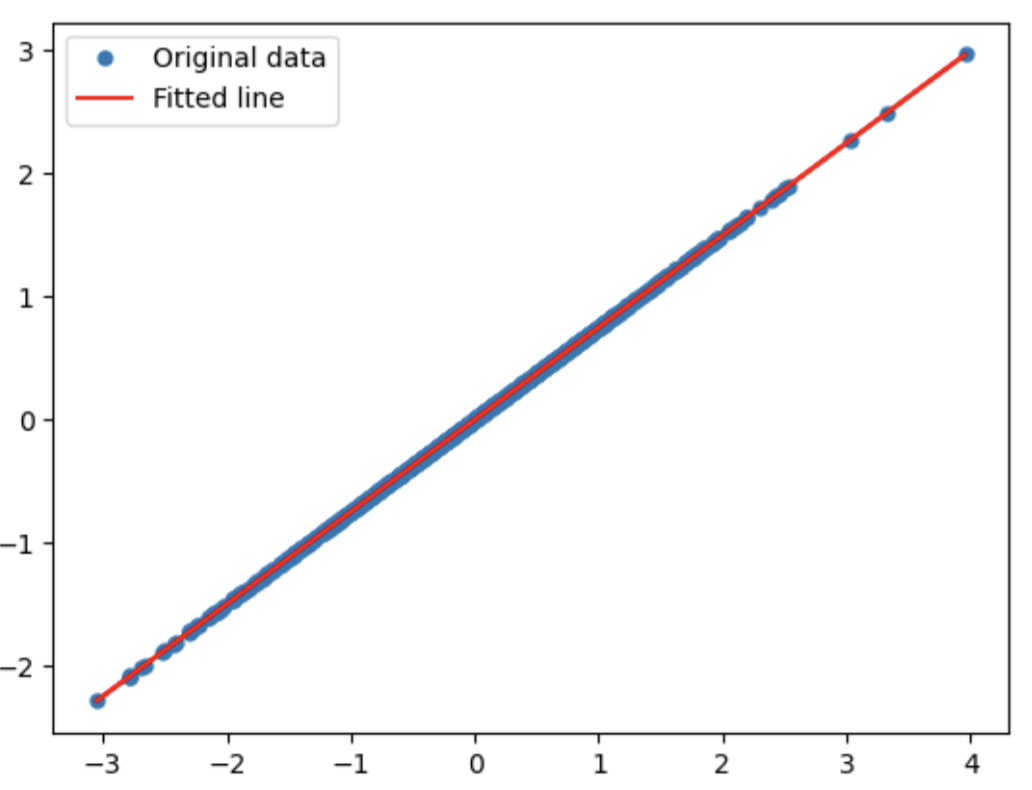
\includegraphics[width=6cm]{images/linearFunctionA.png}
    \caption{Dataset (A) with a linear function}
    \label{linearA}
\end{figure}

Finally regarding to the question why it is not a good idea to use radial basis functions for this dataset is that as we can see in the figure \ref{linearA} the data is linear, so it's obvious that using a linear function to approximate a linear dataset is the best option and the radial basis functions is to approximate nonlinear functions. 

\noindent \textbf{Part 2:} 

In this second part, we have to approximate the function in dataset (B) with a linear function, so as in the previous part, we have minimized the equation \ref{linear} and we have solved it with the least-squares minimization algorithm. In the figure of above we can see our approximated function with the dataset, clearly, it does not fit well. This is due to that our dataset is not linear, so we cannot approximate a nonlinear dataset with a linear function.

\begin{figure}[H]
    \centering
    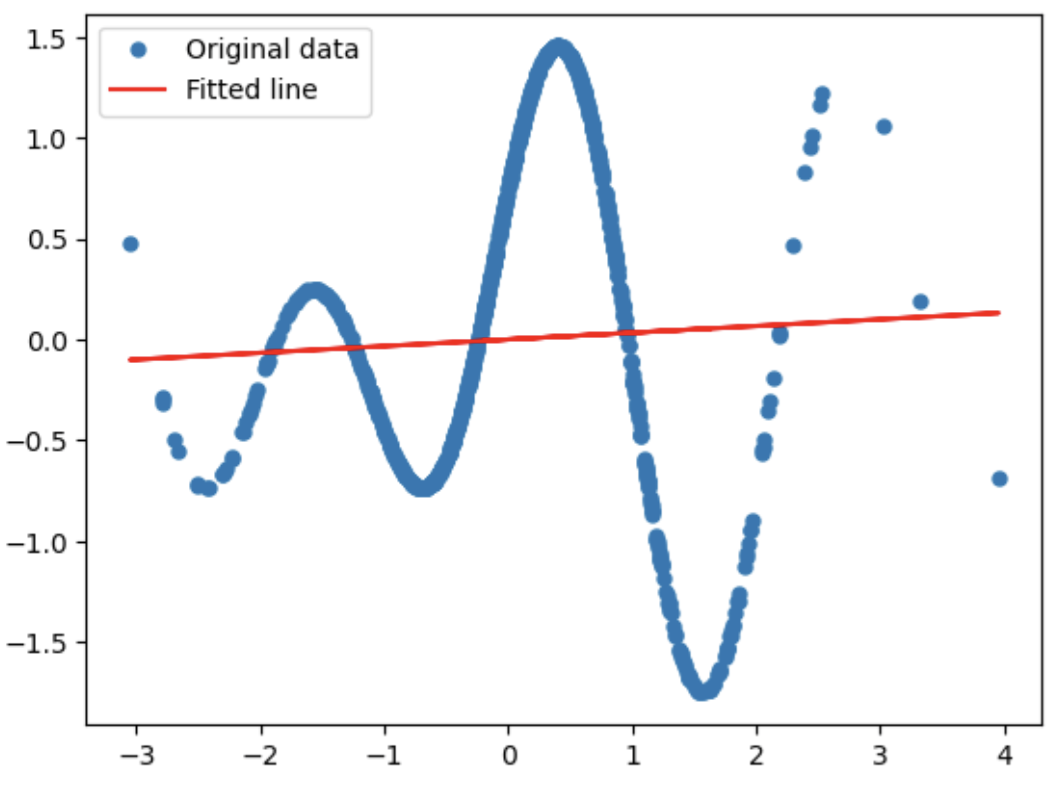
\includegraphics[width=6cm]{images/linearFunctionB.png}
    \caption{Dataset (B) with a linear function}
    \label{linearB}
\end{figure}

\noindent \textbf{Part 3:} 

Finally, in this last part we have to approximate the function in dataset (B) with a combination of radial functions, that turns out to be a nonlinear function. In this case, we have to minimize the equation \ref{nonlinear}. First, we have applied the L radial functions to our dataset (B) and then we have applied the least-squares minimization algorithm to the L transformed dataset. As we can see in the figure above, this function fits much better than the linear function in the previous task.

\begin{figure}[H]
    \centering
    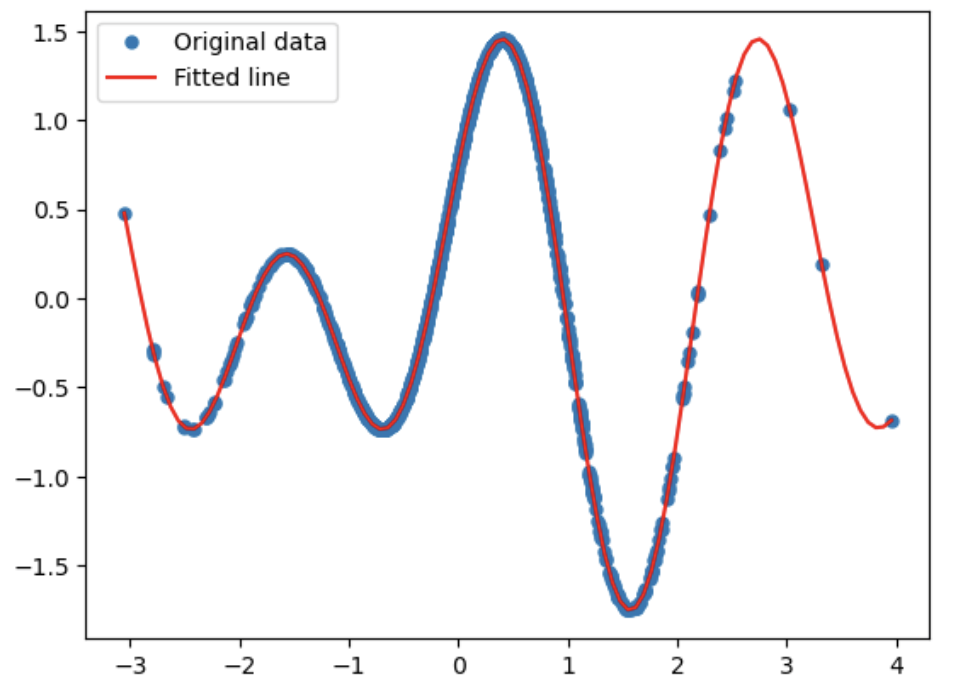
\includegraphics[width=6cm]{images/nonLinearFunctionB.png}
    \caption{Dataset (B) with a nonlinear function}
    \label{nonLinearB}
\end{figure}

The radial basis functions we have created is defined by:

\begin{equation}\label{radial}
    \phi_{l} = \exp (- \| x_{l} - x \| ^ {2} / \epsilon)
\end{equation}

As said in the statement, we have just used a uniformly spaced sampling over the space [$x_{min}$, $x_{max}$], which is the domain where we want to approximate the function to define our center points $x_{l}$. We have use the instruction np.linspace(-$x_{min}$, $x_{max}$, $L$) to define the center points, where L is the number of center points and also the number of radial basis functions we have created. If L is exactly the same as the number of data points, then it will fit perfectly, but it is not what we want because it is causing overfitting on our dataset and generalization, interpolation and extrapolation may not be very good. In our case, we have chosen 50 for the parameter L for 1000 datapoints of our dataset. It is quite small comparing with the number of datapoints, but as we can see in the figure \ref{nonLinearB}, it is performing quite well. And after trying several $\epsilon$'s, we have chosen $\epsilon = 1$, which is the one that performs the best. Also comparing the results of choosing $\epsilon$ or $\epsilon^{2}$ in the denominator for the radial functions, we have gone with $\epsilon$ because it gives better results.

\end{task}

\newpage

\begin{task}{2, Approximating linear vector fields}

In this second task, we have to approximate linear vector fields. For this purpose, we have downloaded the datasets \texttt{linear\_vectorfield\_data\_x0.txt} and \texttt{linear\_vectorfield\_data\_x1.txt} from Moodle. Each of them contains 1000 rows and two columns, for 1000 data points $x_0$ and $x_1$ in two dimensions. This task also contains three parts.

The notebook \texttt{task2.ipynb} has been created to estimate the linear vector fields.

\bigskip

\noindent \textbf{Part 1:} 

In the first part of this task, we have estimated the linear vector field that was used to generate the points $x_1$ from the points $x_0$ (Figure \ref{vector_field}). 

\begin{figure}[H]
    \centering
    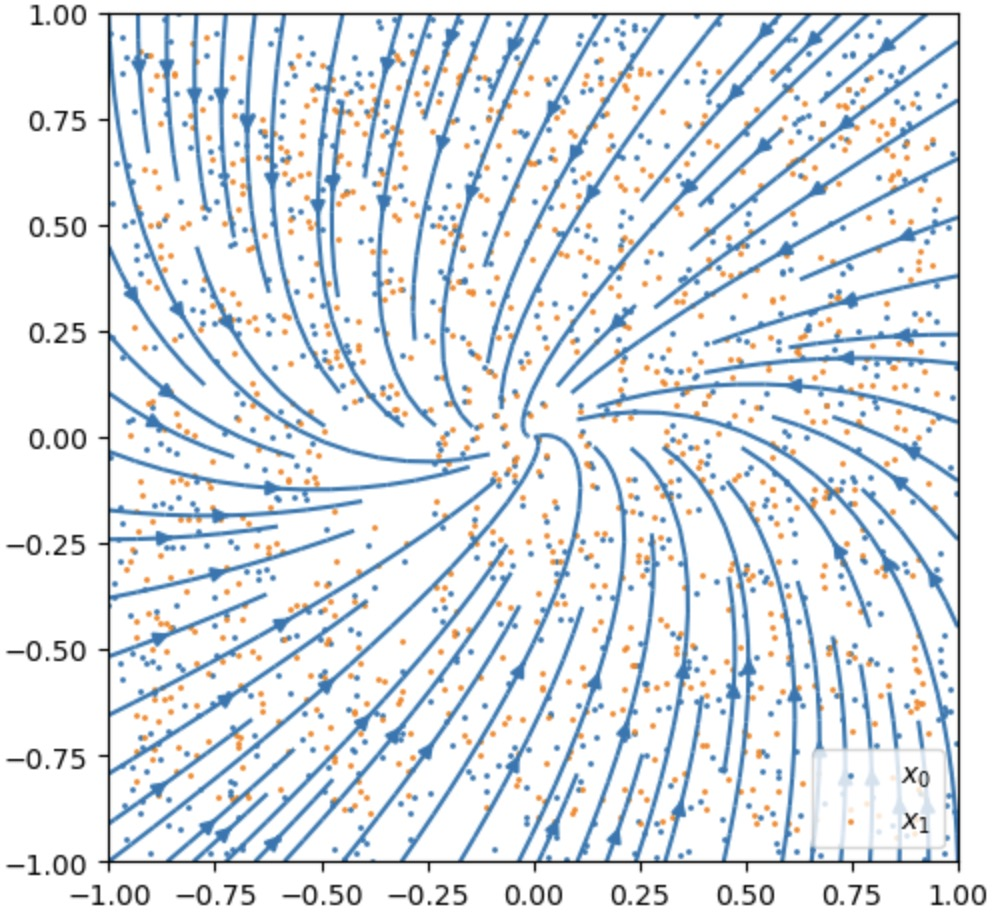
\includegraphics[width=8cm]{images/vector_field.jpg}
    \caption{Estimated linear vector field that was used to generate the points $x_1$ from the points $x_0$}
    \label{vector_field}
\end{figure}

Firstly, we have used the finite-difference formula from the equation \ref{vectorfield} to estimate the vectors $v^{(k)}$ at all points $x_0^{(k)}$, with a time step $\Delta t = 0.1$.

\begin{equation}\label{vectorfield}
    \hat{v}^{(k)} = \frac{\hat{x}^{(k)}_{1} - \hat{x}^{(k)}_{0}}{\Delta t} 
\end{equation}

Then, we have approximated the matrix $A \in \mathbb{R} ^ {2x2}$ with a supervised learning problem, by using the least-squares minimization algorithm. Since the vector field is linear, for all k:

\begin{equation}\label{k}
    \upsilon (\hat{x}^{(k)}_{0}) = \hat{v}^{(k)} = A \hat{x}^{(k)}_{0}
\end{equation}

\noindent \textbf{Part 2:} 

In the second part, we have solved the linear system $\dot{x} = \hat{A} x$, where $\hat{A}$ is the approximated matrix we have found in the previous part, such that $\hat{A} \approx A$, with all ${x}^{(k)}_{0}$ as initial points, up to a time $T_{end} = \Delta t = 0.1$. Then we got the estimates for the points $x^{(k)}_{1}$. The linear system has been solved in two different ways: with the Euler's method's approach and using the method \texttt{integrate.solve\_ivp} of the Python library and, since this second method is a more accurate integration method, it will be used for the next tasks as well. Once we got $\hat{x}^{(k)}_{1}$ (the estimates of $x^{(k)}_{1}$), we have computed the mean squared error to all the known points $x^{(k)}_{1}$ with the following formula:

\begin{equation}\label{mse}
    \frac{1}{N} \sum_{k=1}^{N} \| \hat{x}^{(k)}_{1} - x^{(k)}_{1} \| ^ {2}
\end{equation}

\noindent with N = 1000. The error of our estimation is \num{3.06e-3}, which is small enough to conclude that approximating the vector field using a linear approach was a good choice (as expected), and that it was correctly approximated.

\newpage

\noindent \textbf{Part 3:} 

In the last part of this task, we solved again the linear system $\dot{x} = \hat{A} x$ with our matrix approximation, but now with a initial point (10, 10), far outside the initial data and for $T_{end} = 100$. In this case, for the trajectory, we have used the Euler's method as it was the method provided in the previous exercise. Then we have plotted the trajectory as well as the phase portrait in a domain $[-10, 10]^{2}$ as we can see in the Figure \ref{pahse_portrait}. 

\begin{figure}[H]
    \centering
    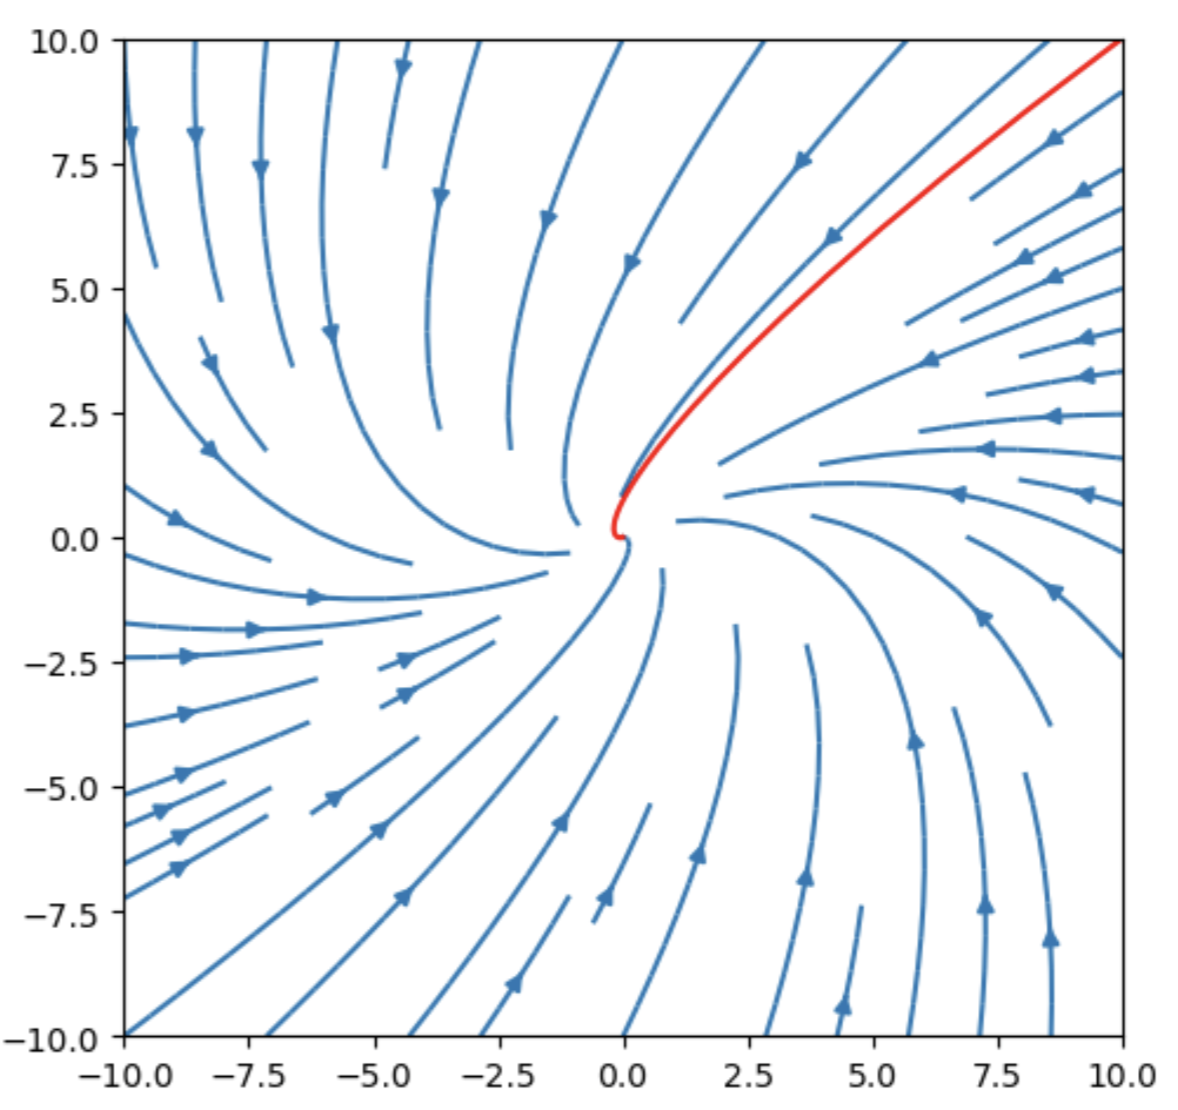
\includegraphics[width=8cm]{images/phase_portrait.png}
    \caption{Phase portrait with a trajectory in the domain $[-10, 10]^{2}$}
    \label{pahse_portrait}
\end{figure}

We can observe that there is a attractive steady state in the origin (0, 0) in the phase portrait and the red line is the trajectory that the initial point at (10, 10) follows to reach the steady state.

\end{task}

\newpage

\begin{task}{3, Approximating nonlinear vector fields}

After approximating linear vector fields, in this task we have to approximate now nonlinear vector fields using the datasets \texttt{nonlinear\_vectorfield\_data\_x0.txt} and \texttt{nonlinear\_vectorfield\_data\_x1.txt}. These datasets contains each of them 2000 rows and two columns, for 2000 data points $x_0$ and $x_1$ in two dimensions.

The first dataset contains the initial points $x_{0}$ over the domain $[-4.5, 4.5]^{2}$, while the second one contains the same points advanced with an unknown evolution operator $\psi : T \times \mathbb{R} ^ {2} \rightarrow \mathbb{R} ^ {2}$, such that:

\begin{equation}\label{psi}
    x^{(k)}_{1} = \psi (\Delta t, x^{(k)}_{0}),   k = 1,...,N
\end{equation}
 
\noindent with a small $\Delta t = 0.01$, i.e., smaller than in the task on linear vector fields.

The notebook \texttt{task3.ipynb} has been created to cover this task, which has three parts as well.

\bigskip

\noindent \textbf{Part 1:} 

As in the previous task, in this first part we have to estimate the vector field describing $\psi$ with a linear operator $A \in \mathbb{R} ^ {2x2}$, such that 

\begin{equation}\label{linearoperator}
    \frac{d}{ds} \psi(s, x(t)) \biggm| _{s = 0} \approx \hat{f}_{linear}(x(t)) = Ax(t).
\end{equation}

For estimating the vector field $A$ we have used once again the least-squares minimization algorithm. The phase portrait of this vector field alongside the points $x_0$ and $x_1$ can be observed in Figure \ref{non_linear_vector_field}.

\begin{figure}[H]
    \centering
    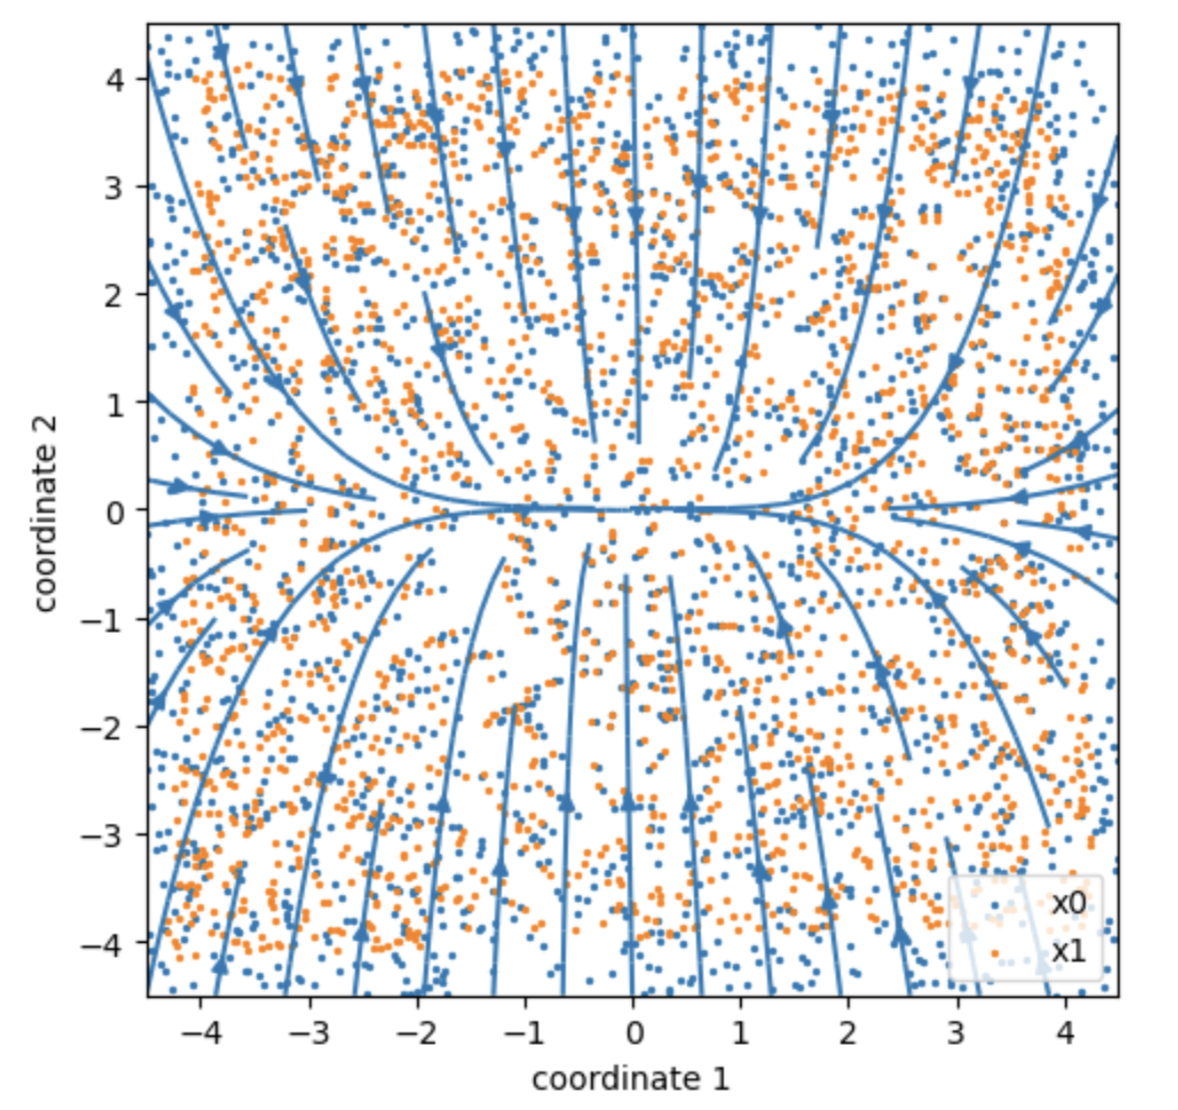
\includegraphics[width=8cm]{images/non_linear_vector_field.png}
    \caption{Estimated vector field with a linear operator}
    \label{non_linear_vector_field}
\end{figure}

Once we have obtained $A$, we have to check now how good was the approximation by calculating the mean squared error between all the approximated and known end points. Since we had applied the finite-difference formula with $\Delta t = 0.01$ for estimating $A$, it is logical to choose it again for integrating the linear system in order to obtain the approximated end points $\hat{x}^{(k)}_{1}$ as close as possible to the known end points $x^{(k)}_{1}$.

The mean squared error between all the approximated end points and the known end points for $\Delta t = 0.01$ is equal to \num{3.729e-2}, which is small but pretty big compared to the error obtained in the previous task.

\newpage

\noindent \textbf{Part 2:} 

Now, we have to estimate the vector field using radial basis functions, such that 

\begin{equation}\label{rbf}
    \frac{d}{ds} \psi(s, x(t)) \biggm| _{s = 0} \approx \hat{f}_{rbf}(x(t)) = C\phi(x(t)).
\end{equation}

The central points have been equally distributed all over the domain $[-4.5, 4.5]^{2}$. For choosing the number of central points $L$, we have tried different values between 100 and 1000 and we have stuck with the one that minimized the mean squared error later on, which was 100. Moreover, choosing a relatively small number compared to the number of points is a good option for achieving a good generalization and reducing the execution time. As for $\epsilon$, the value that minimized the MSE was $\epsilon = 0.75$ (not squared).

Having the radial basis functions $\phi(X)$ defined and applied to all points $x_0$, we obtained the coefficient matrix $C$ using the least-squares minimization algorithm. For visualizing the phase portrait of this new vector field, the function $\hat{f}_{rbf}(x(t)) = C\phi(x(t))$ has been applied to several points equally distributed over the domain in order to obtain the approximated vector in each point. The phase portrait alongside the points $x_0$ and $x_1$ is displayed in figure \ref{nonlinear_vector_field2}. Note that this new nonlinear vector field fits much better the dataset points than the linear one.

\begin{figure}[H]
    \centering
    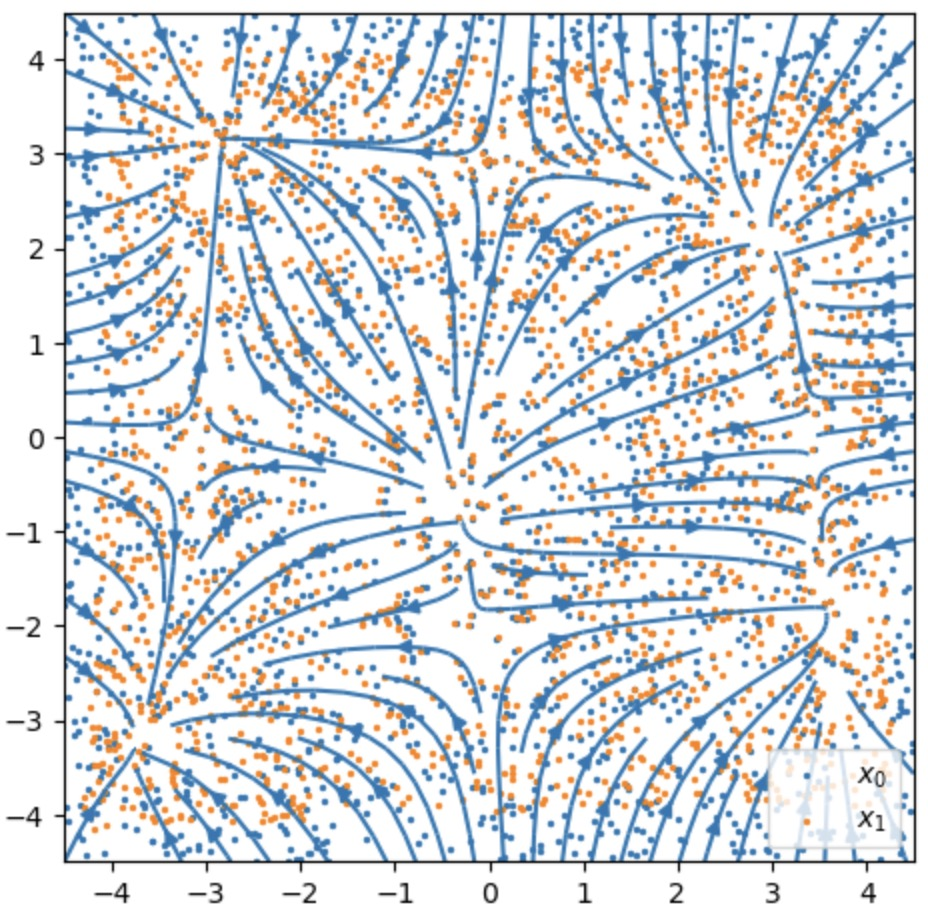
\includegraphics[width=8cm]{images/nonlinear_vector_field2.jpg}
    \caption{Estimated vector field using radial basis functions}
    \label{nonlinear_vector_field2}
\end{figure}

Let's check again how good was the approximation by using the same methodology as in the previous part, but now integrating the linear system given by $\dot x = C\phi(x(t))$. The mean squared error is now equal to \num{6.731e-4}, which is significantly smaller compared to the error obtained in the last part, where we used a linear approximation. With this we can conclude that the vector field is nonlinear, as a more precise vector field has been obtained with a nonlinear approximation.

\newpage

\noindent \textbf{Part 3:}

In this last part we were asked to figure out where are the steady states of the system we have chosen, which is the nonlinear one.

For this, we have used the approximated vector field to solve the system for a larger time, with all initial points $x_0$. All points $x_0$ converged into four steady states for a time $\Delta t = 5$, in the positions shown in Figure \ref{steady_states}. Since this nonlinear system has multiple steady states, it cannot be topologically equivalent to a linear system.

\begin{figure}[H]
    \centering
    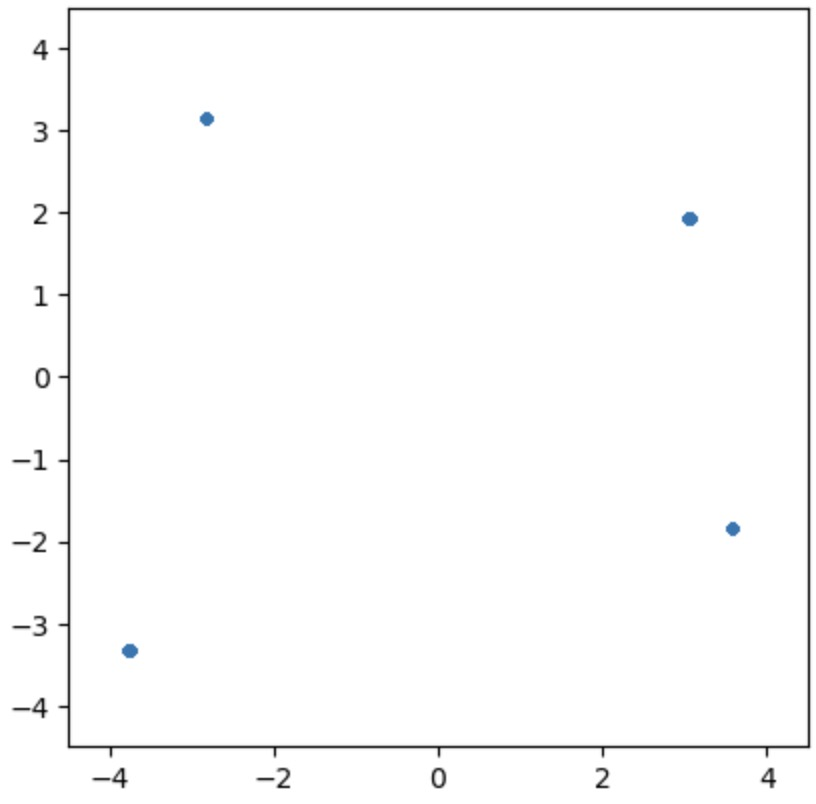
\includegraphics[width=8cm]{images/steady_states.jpg}
    \caption{Steady states of the nonlinear vector field}
    \label{steady_states}
\end{figure}

\end{task}

\newpage

\begin{task}{4, Time-delay embedding}
\subsubsection*{Part 1: Embedding periodic signal into state space}
In this task we embed a periodic signal into a state space where each point carries
enough information to advance in time. After loading the \texttt{takens\_1.txt} dataset we plot the datapoints in 2D-space and the first coordinate $x_0(t)$ against time (row number).

\begin{figure}[H]
    \centering
    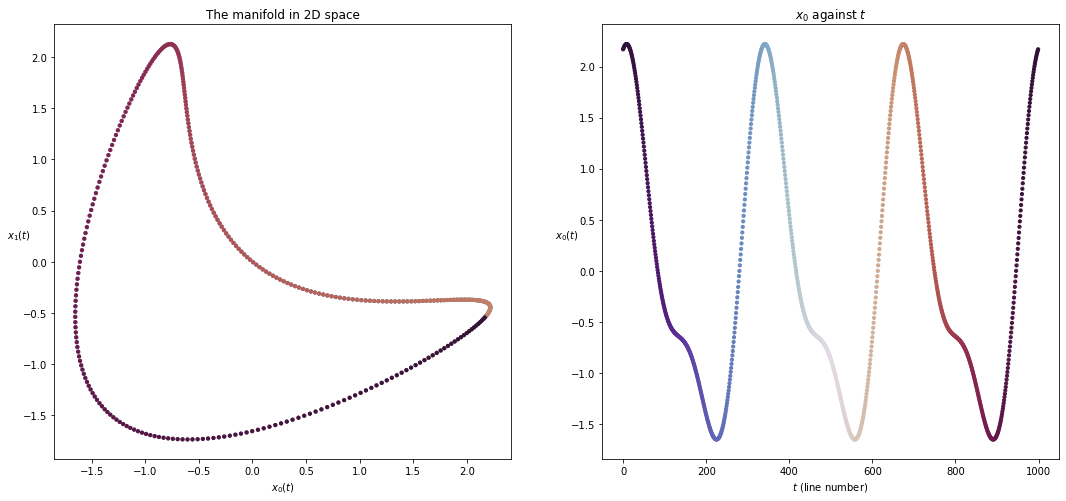
\includegraphics[width=14cm]{images/task4-1-0.png}
    \caption{Signal datapoints in 2D-space and the first coordinate $x_0(t)$ against time.}
    \label{task4-1-0}
\end{figure}

Now, we take the coordinate $x_0$, and plot it against its delayed version, $x_0(n+\Delta n)$, where $\Delta n$ is the number of lines by which the coordinate is shifted. In the first graph we plot the first coordinate $x_0(t)$ against its delayed version $x_0(t-\Delta n)$, where $\Delta n$ is the number of rows (time) by which $x_0(t)$ is delayed. 

At the same time, according to Takens theorem we only need 2 more coordinates to plot that the 1d series $x_0(t)$ is sure to be embedded correctly. We can use a smooth diffeomorphism $\psi: \mathbb{R} \rightarrow \mathbb{R}$ defined as a shift operation $$\psi(t) = t-\Delta n$$ 
and the map $E_{(\psi, x_0)}: \mathbb{R} \rightarrow \mathbb{R}^3$ defined as $$E_{(\psi, x_0)}(t)=\left(x_0(t), x_0(\psi(t)), x_0(\psi(\psi(t)))\right)$$ to embed $x_0(t)$ from $\mathbb{R}$ into $\mathbb{R}^3$.

In the second graph the three line correspond with the three embedded coordinates $x_0(t), x_0(\psi(t)), x_0(\psi(\psi(t)))$ against time $t$, and in the last is the embedded vector result plotted in 3D space.

We also plot the results for the second coordinate $x_1(t)$, along with which there are 6 coordinates have we used in total to sufficiently display the charateristics of the entire periodic manifold. 

Results for this part are showing in figure \ref{task4-1-1} on the next page.

\begin{figure}[H]
    \centering
    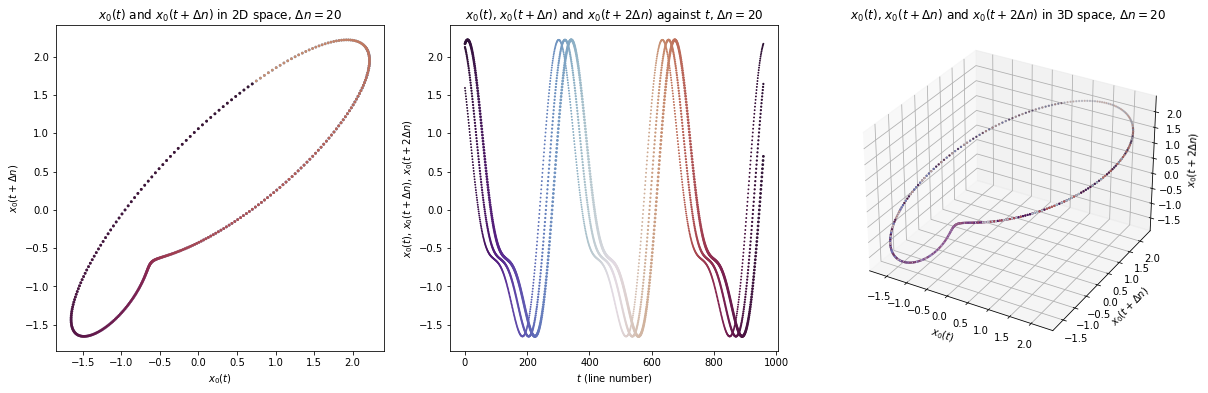
\includegraphics[width=16cm]{images/task4-1-1-20.png}
    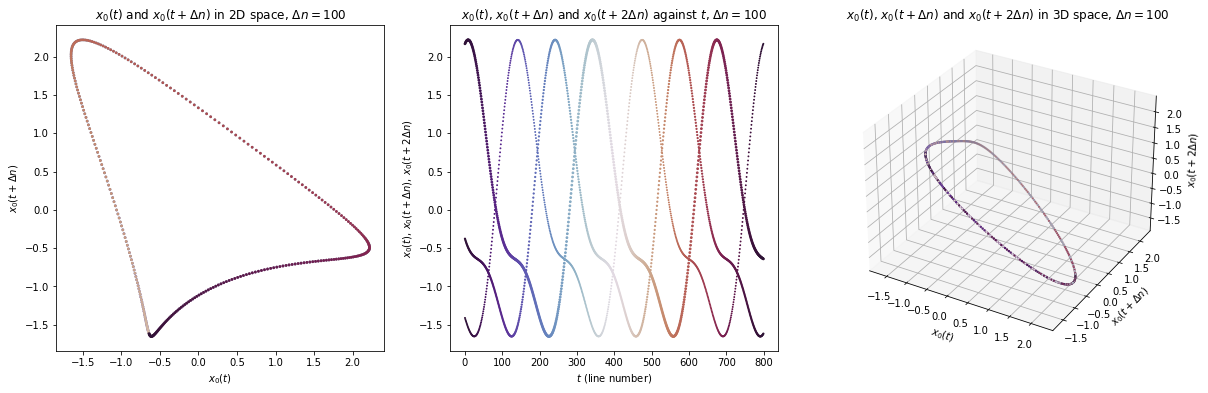
\includegraphics[width=16cm]{images/task4-1-1-100.png}
    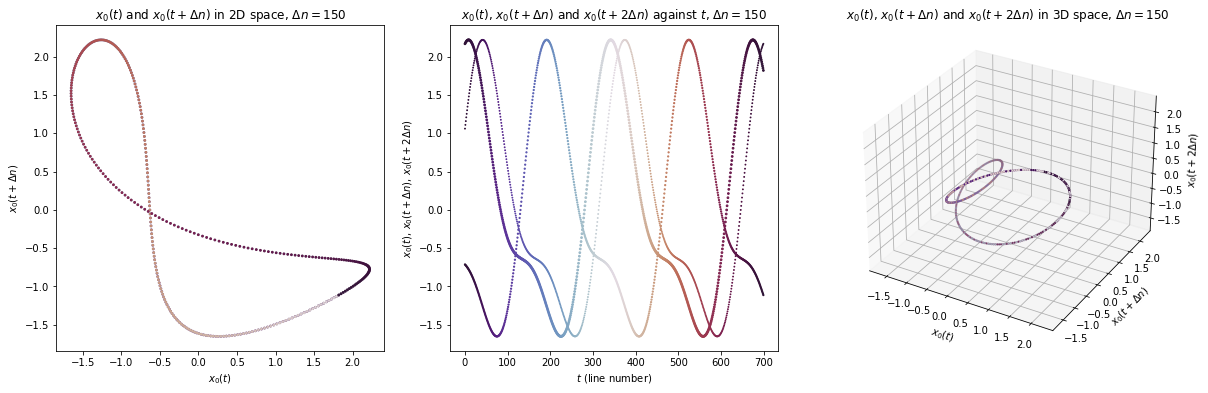
\includegraphics[width=16cm]{images/task4-1-1-150.png}
    \caption{Shifted results for using $\Delta n=20, 50, 100$} 
    \label{task4-1-1}
\end{figure}

\bigskip

\subsubsection*{Part 2: Approximating chaotic dynamics from time series}

In this task we test the Takens theorem and our results on the Lorenz system. For a Lorenz system with $\sigma=10, \rho=28, \beta=\frac{8}{3}$, we split the calculated trajectories into its three coordinates and observe the behavior of each. By using Takens theorem and the shift operations similarly, we can embed each coordinates' projections of trajectory into 3 variables as aforementioned. The result is simulated with $T_{end}=20$ seconds and simulation step length $\text{d}t=0.001$ second.

Results on variables $x$ and $z$ are showing in figure \ref{task4-2-x} and \ref{task4-2-z} on the following pages.

\begin{figure}[H]
    \centering
    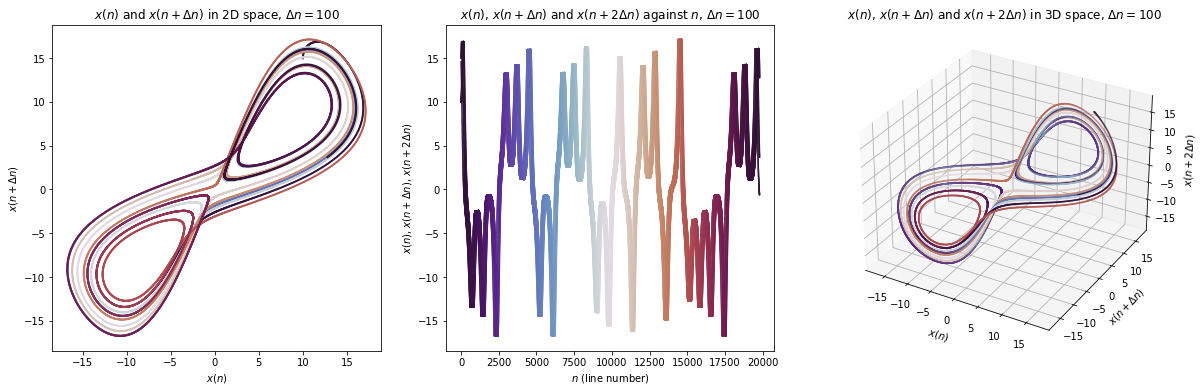
\includegraphics[width=16cm]{images/task4-2-x-0.1.png}
    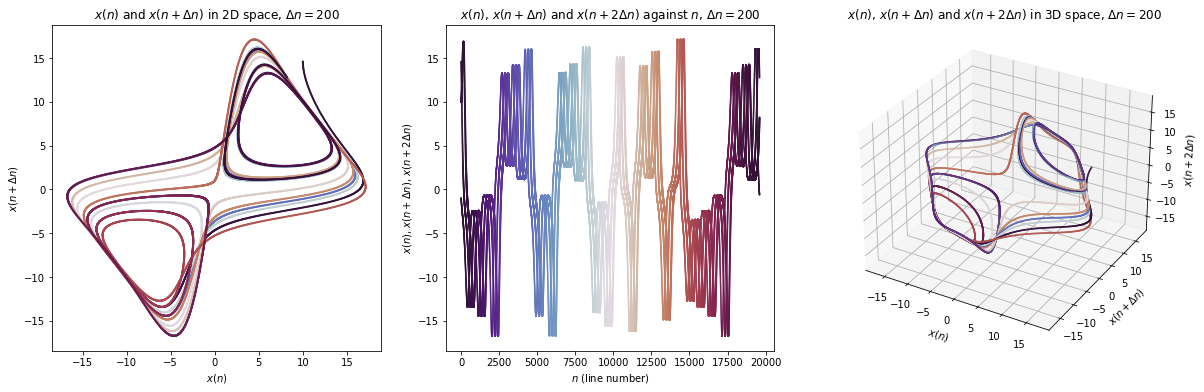
\includegraphics[width=16cm]{images/task4-2-x-0.2.png}
    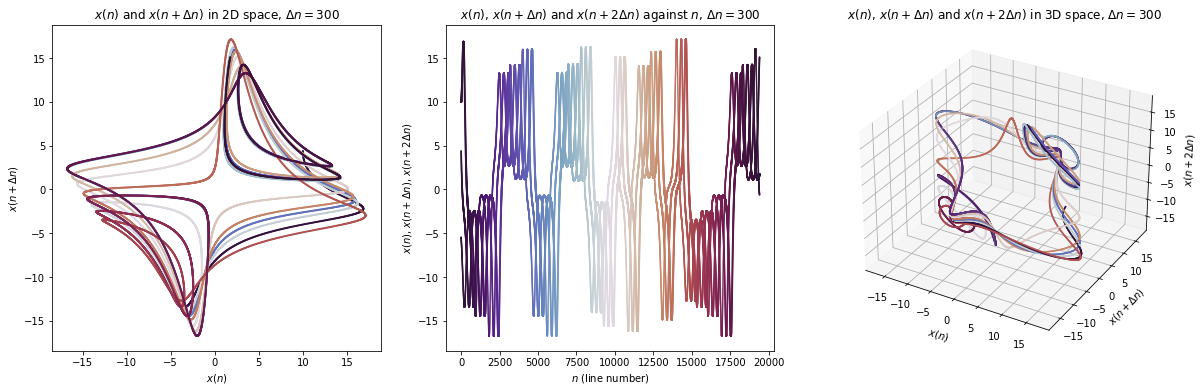
\includegraphics[width=16cm]{images/task4-2-x-0.3.png}
    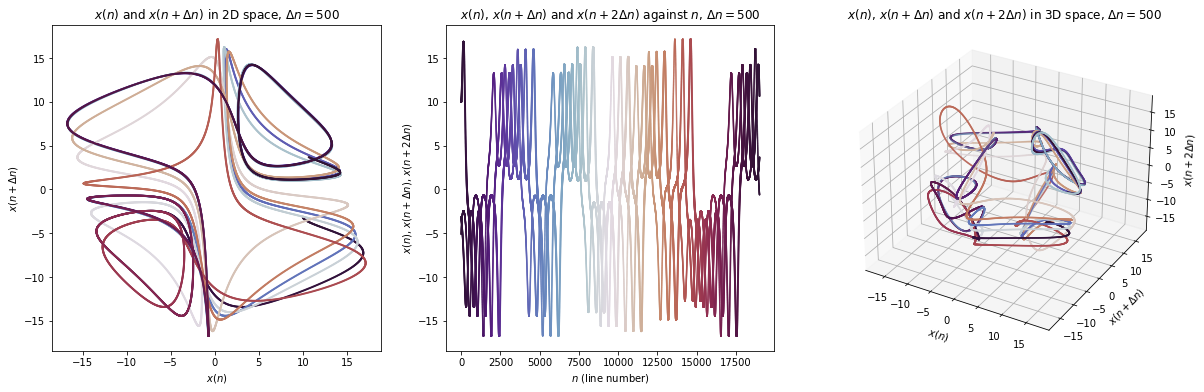
\includegraphics[width=16cm]{images/task4-2-x-0.5.png}
    \caption{Shifted results for the trajectory's $x$ coordinate in the Lorenz system, using $\Delta t=0.1, 0.2, 0.3, 0.5$}
    \label{task4-2-x}
\end{figure}

\begin{figure}[H]
    \centering
    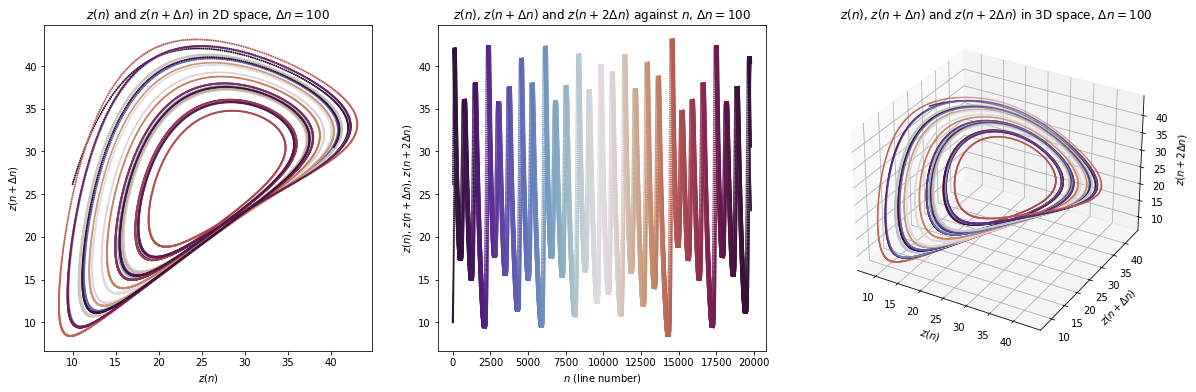
\includegraphics[width=16cm]{images/task4-2-z-0.1.png}
    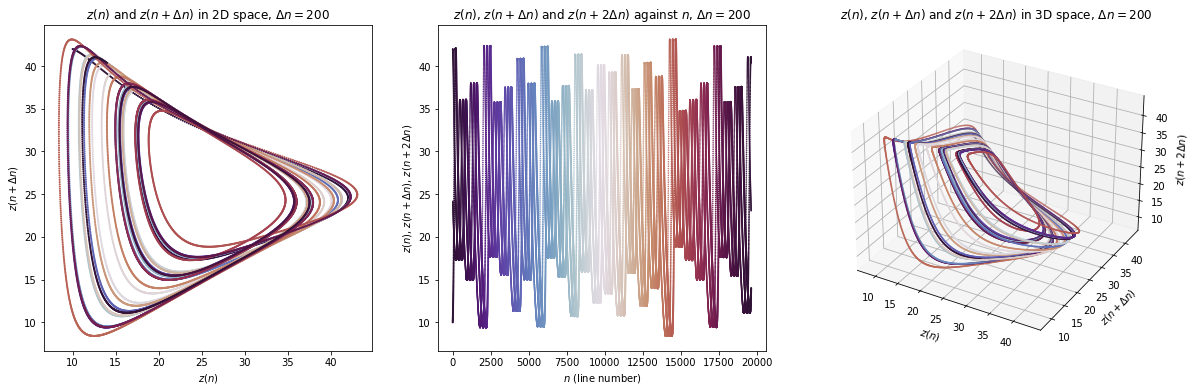
\includegraphics[width=16cm]{images/task4-2-z-0.2.png}
    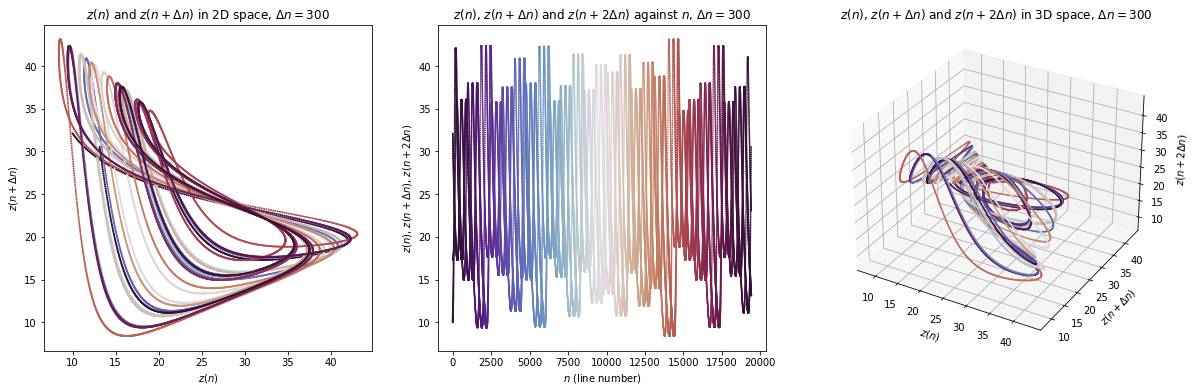
\includegraphics[width=16cm]{images/task4-2-z-0.3.png}
    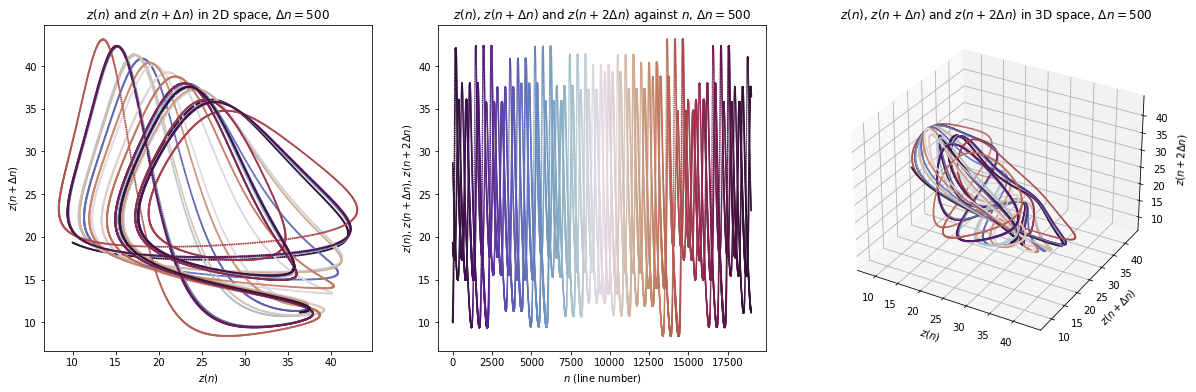
\includegraphics[width=16cm]{images/task4-2-z-0.5.png}
    \caption{Shifted results for the trajectory's $z$ coordinate in the Lorenz system, using $\Delta t=0.1, 0.2, 0.3, 0.5$}
    \label{task4-2-z}
\end{figure}

From the results we can tell that embedding works for $x$ and fails for $z$. The shape we got for $x$ with using suitable $\Delta_t$ is similar to the original butterfly shape and captured the characteristics of the two attractors, whereas for $z$ we only have a circling shape. We further certify this by testing for $y$ in figure \ref{task4-2-y} where we could see that it also works.

\begin{figure}[H]
    \centering
    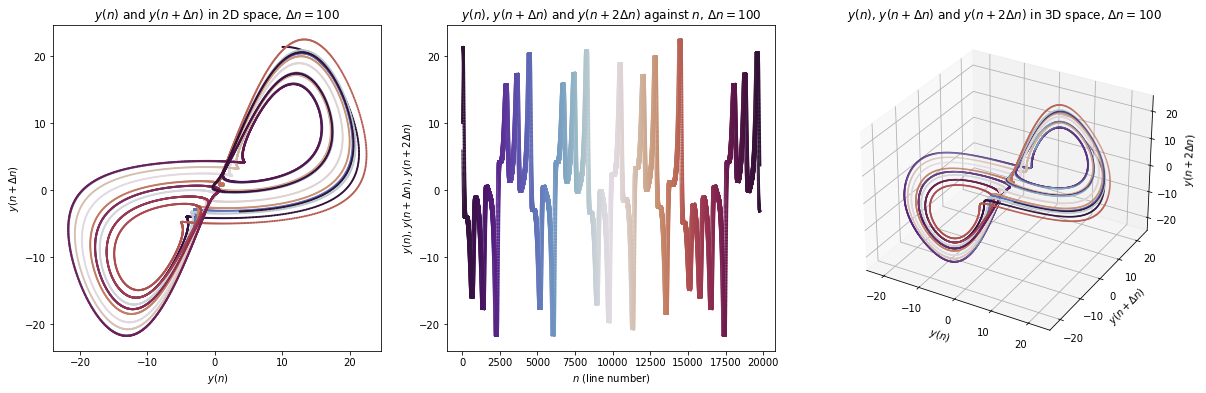
\includegraphics[width=16cm]{images/task4-2-y-0.1.png}
    \caption{Shifted results for the trajectory's $y$ coordinate in the Lorenz system, using $\Delta t=0.1$}
    \label{task4-2-y}
\end{figure}

By observing the middle subplot in the figures, we could tell the reason why time-delay embedding for the $z$ coordinate fail to capture the behaviorism with attractor is because that the $z$-axis component of the original butterfly trajectory does not contain information about the bifurcation behavior at the beginning. The system's position on $z$-axis keeps orbiting within a same range of values, whereas on $x$ and $y$ axis could it exhibit the behavioral pattern of alternately oscillating around two different attractors. 

\begin{figure}[H]
    \centering
    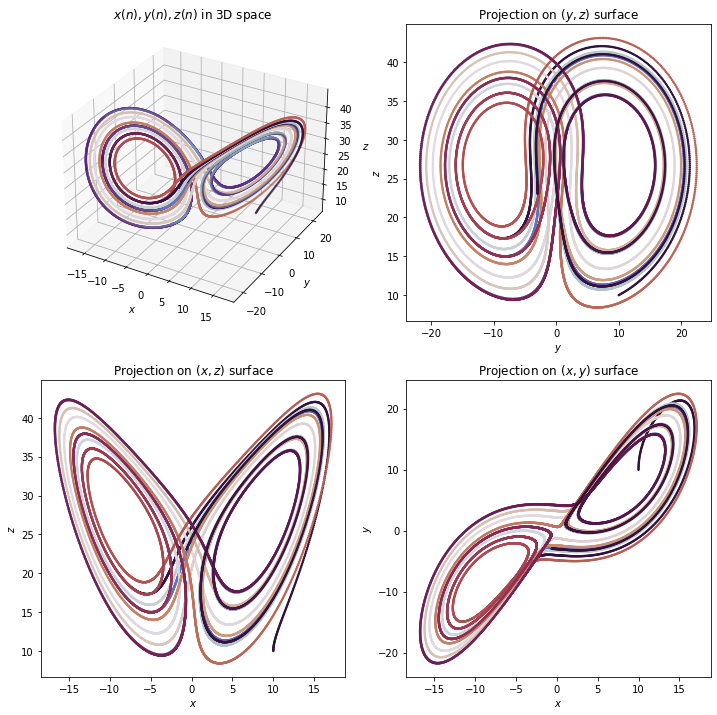
\includegraphics[width=12cm]{images/task4-2-lorenz.png}
    \caption{The trajectory and its projections in the Lorenz system}
    \label{task4-2-lorenz}
\end{figure}

This reasoning can also be observed in the original 3D plot of the Lorenz attractor, where we can see that the underlying reason behind this phenomenon is that the centroids' position of the two attractors shares almost the same $z$ value, but distinctively not $x$ and $y$. In this way the system cannot tell which attractor the system is currently engaged with by only using information on the $z$ axis.

\subsubsection*{Bonus: Approximation of vector field for the Lorenz attractor}

In the bonus task we take the shifted $x$-coordinate to approximate the vector field $\hat{\nu}$ of the Lorenz-attractor, and plot the shifted vector field from its starting positions in a quiver plot. After concatenating the values of coordinated $x(t), x(t+\Delta t)$ and $x(t+2\Delta t)$ together we calculate the vectors pointing from data points to their corresponding targets, which is shifted using another $\Delta n=1$. Hereby the process behaves as the computation of the approximation through the radial basis functions.

\begin{figure}[H]
    \centering
    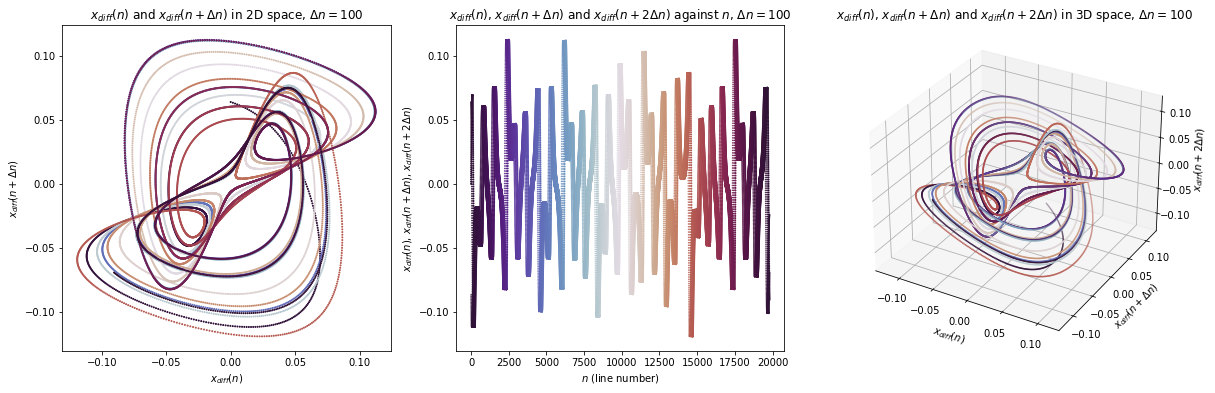
\includegraphics[width=13cm]{images/task4-3-1.png}
    \caption{The medium results of the vectors pointing from data points to corresponding targets}
    \label{task4-3-1}
\end{figure}

We proceed creating a quiver plot showing reconstructed vector field in 3D space from their starting locations, obtaining similar graph to the embedding of the attractor with the $x$ coordinate.

\begin{figure}[H]
    \centering
    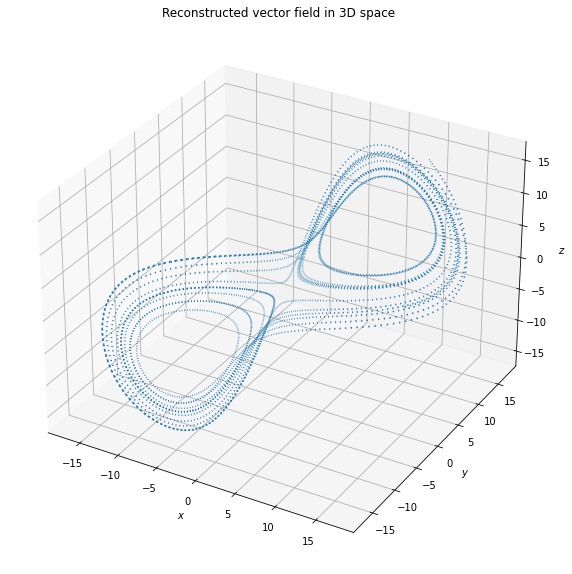
\includegraphics[width=11cm]{images/task4-3-2.png}
    \caption{The reconstruction of the $x$ coordinate time delay embedding of the Lorenz attractor}
    \label{task4-3-2}
\end{figure}

\end{task}

\newpage

\begin{task}{5, Learning crowd dynamics}
The last task is centered on learning a dynamical system describing the people flow in nine different areas of TUM Garching, containing the MI Building and the 2 mensas. The given database describes the system over the course of 7 days and is divided as follows: it has a first column containing the time index (which is simply a natural number going up one by one and starting from 1) and 9 other columns containing the number of people per area at that certain time. 

\subsubsection*{Part 1:}
After loading and exploring data we already know the dataset being periodic with the same pattern and no parametric dependence, therefore can be reduced to become 1-dimensional. Following Takens theorem we can assert to construct an embedding with 3 dimension to get a reasonable state space. 

\begin{figure}[H]
    \centering
    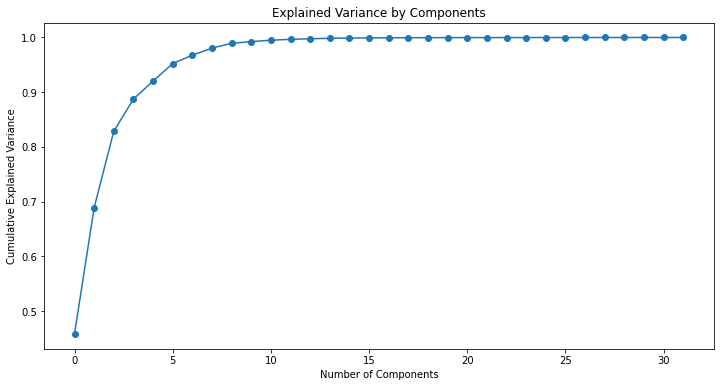
\includegraphics[width=12cm]{images/task5-1-PCA.png}
    \caption{The cumulative explanined variance using different number of principle components}
    \label{5-1-PCA}
\end{figure}
For PCA, we test the cumulative explained variance by using different number of components, so as to select a most suitable parameter. By which we can see that only using 3 principal components can we represent the state of the system with $83\%$ of the energy now.

\begin{figure}[H]
    \centering
    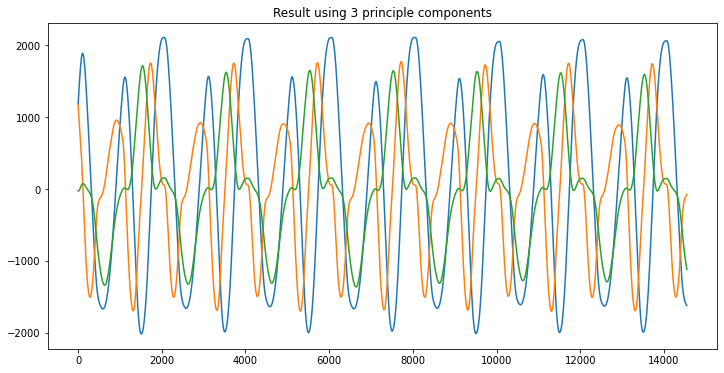
\includegraphics[width=12cm]{images/task5-1.png}
    \caption{The PCA embedded result with 3 principle components}
    \label{5-1}
\end{figure}

We can also plot the result in 3D space with each dimensions representing one principle component.

\begin{figure}[H]
    \centering
    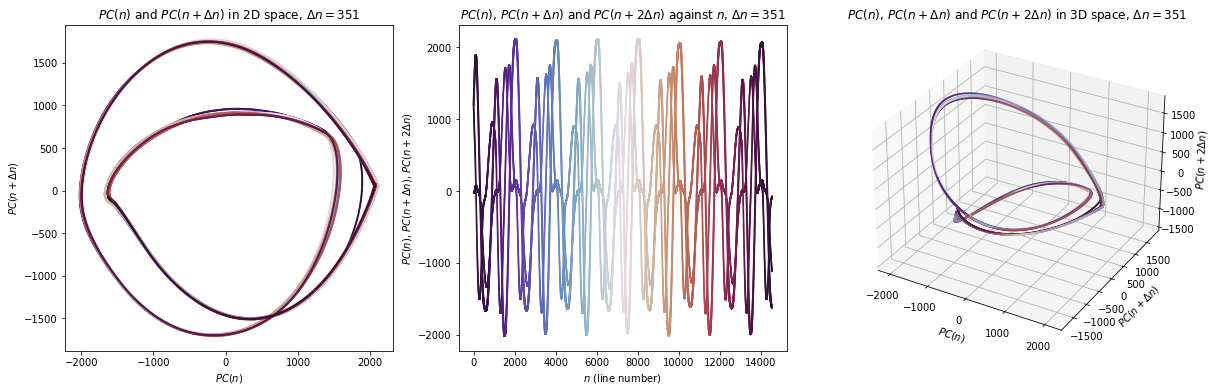
\includegraphics[width=15cm]{images/task5-1-2.png}
    \caption{The PCA embedded result with 3 principle components in 3D space}
    \label{5-1-2}
\end{figure}


\subsubsection*{Part 2:}
For the second part we color the data points by all measurements taken at the first time point of the delays into 9 plots where all the points will be in the same position, only the color changes. This can be achieved by passing different columns as coloring parameter for plotting scatter points.

\begin{figure}[H]
    \centering
    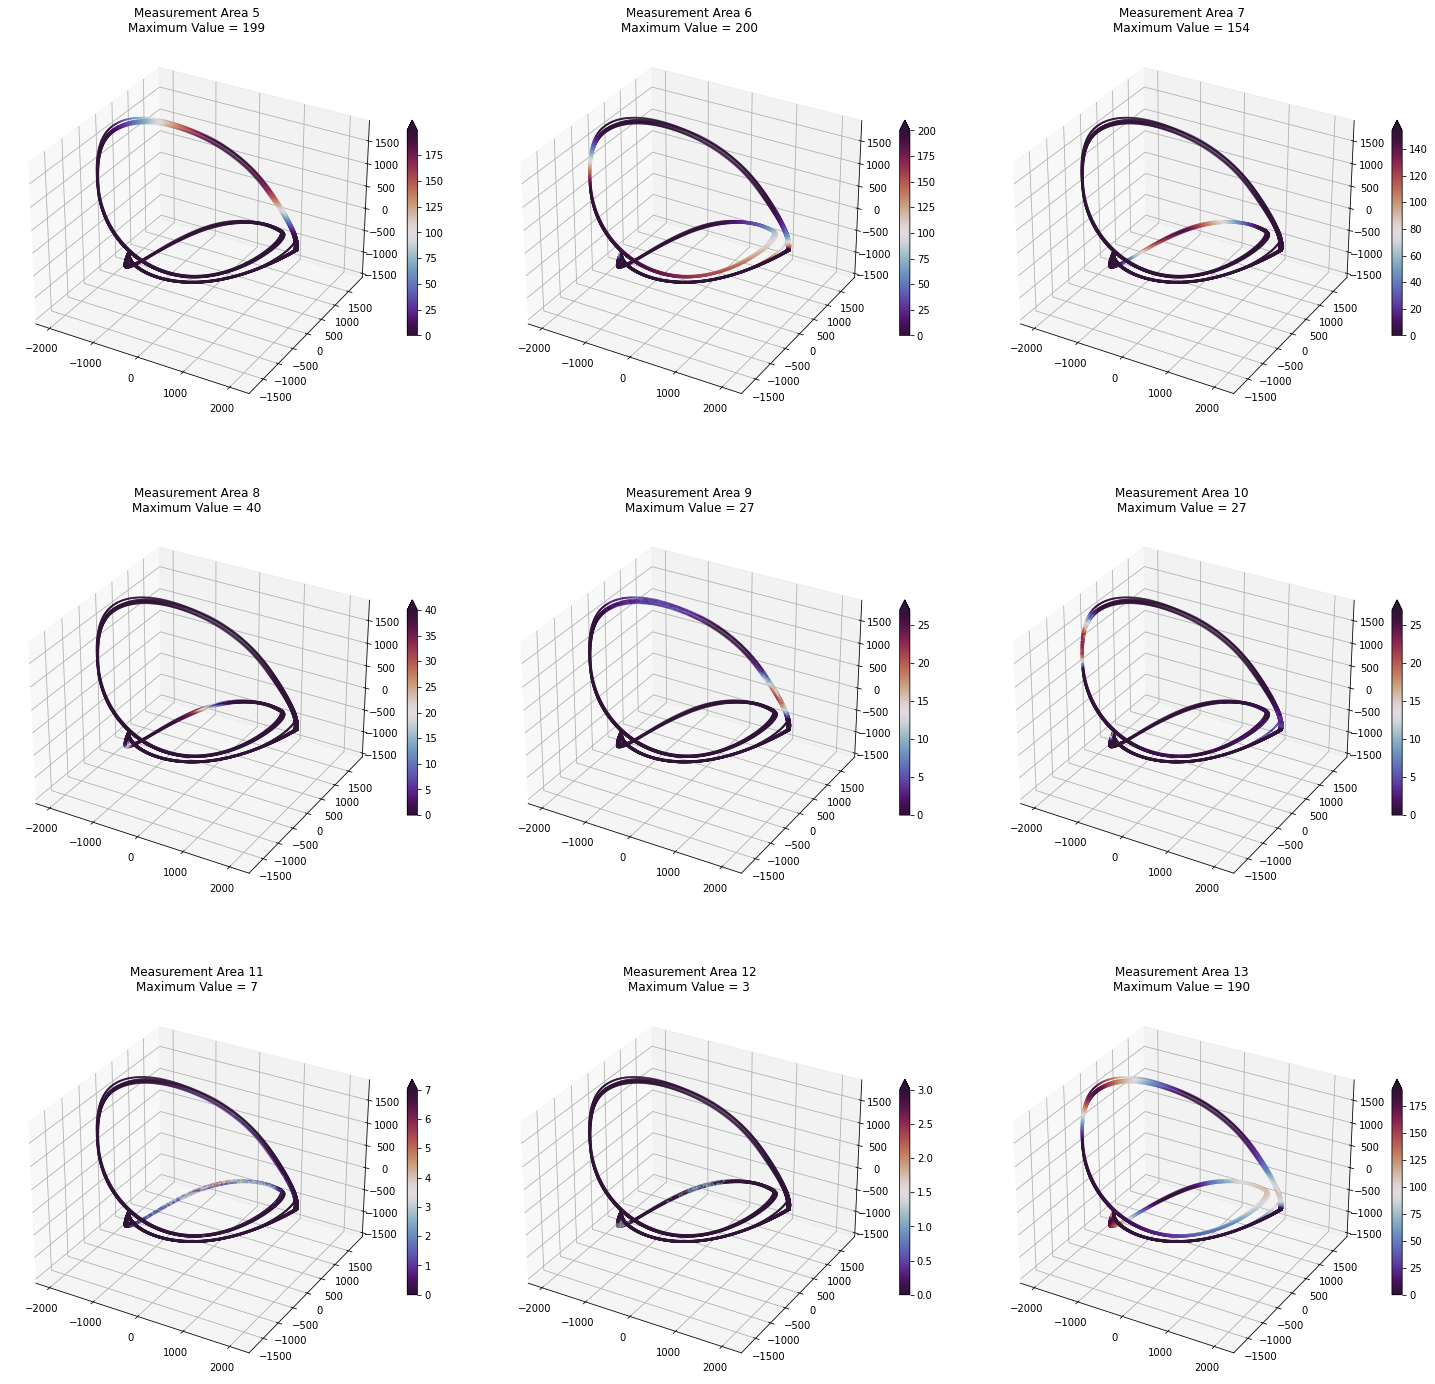
\includegraphics[width=15cm]{images/task5-2.png}
    \caption{The PCA embedded result with 3 principle components in 3D space}
    \label{5-2}
\end{figure}


\subsubsection*{Part 3:}

In this part we want to learn the dynamics on the periodic curve we embedded in the principal components above by computing the arclength of the curve in the PCA space and then approximate the change of arclength over time. 

By observing figure \ref{5-1-PCA} we can tell that a periodicity around every 2000 time step (row numbers) exists for all three components. Hence we calculate the velocity of the arc length by determining how fast the system advances over the PCA space at every point in the space, and then approximate the change in arclength over time. We do this by comparing each time step with the previous one, and use our previously implemented RBF to approximate the velocity. As the data is perodic we only need to do this for the first 2000 data points.


\begin{figure}[H]
    \centering
    \includegraphics[width=15cm]{images/task5-3-RBF.png}
    \caption{The velocity (vector field) result to arclength, with RBF approximation}
    \label{5-3}
\end{figure}

We tested the combinations of different $L$ and $\epsilon$ and selected the current $L=100, \epsilon=0.2$ as it could generate sufficient result efficiently.

\bigskip







\end{task}


\bibliographystyle{plain}
\bibliography{Literature}

\end{document}